%%%%%%%%%%%%%%%%%%%%%%%%%%%%%%%%%%%%%%%%%%%%%%%%%%%%%%%%%%%%%%%%%%%%%%%%%%
%%%%%                         CHAPITRE 4                            %%%%%%
%%%%%%%%%%%%%%%%%%%%%%%%%%%%%%%%%%%%%%%%%%%%%%%%%%%%%%%%%%%%%%%%%%%%%%%%%%

\lhead[\fancyplain{}{\leftmark}]%Pour les pages paires \bfseries
      {\fancyplain{}{}} %Pour les pages impaires
\chead[\fancyplain{}{}]%
      {\fancyplain{}{}}
\rhead[\fancyplain{}{}]%Pour les pages paires 
      {\fancyplain{}{\rightmark}}%Pour les pages impaires \bfseries
\lfoot[\fancyplain{}{}]%
      {\fancyplain{}{}}
\cfoot[\fancyplain{}{\thepage}]%\bfseries
      {\fancyplain{}{\thepage}} %\bfseries
\rfoot[\fancyplain{}{}]%
     {\fancyplain{}{\scriptsize}}


%%%%%%%%%%%%%%%%%%%%%%%%%%%%%%%%%%%%%%%%%%%%%%%%%%%%%%%%%%%%%%%%%%%%%%%%%%
%%%%%                      Start part here                          %%%%%%
%%%%%%%%%%%%%%%%%%%%%%%%%%%%%%%%%%%%%%%%%%%%%%%%%%%%%%%%%%%%%%%%%%%%%%%%%%

\chapter{Robustness assessment}
\label{ch:4}

%==============================================================================	Résumé du chapitre

\begin{center}
\rule{0.7\linewidth}{.5pt}
\begin{minipage}{0.7\linewidth}
\smallskip

\textit{A markerless motion capture method is satisfying if it is accurate, fast, and robust. Robustness is deemed good when results are unchanged while adding constraints on the subject or on the environment. We challenge our workflow on walking, running, and cycling tasks, by adding people in the background, and by simulating challenging conditions: (Im) alters image quality (11-pixel Gaussian blur and 0.5 gamma compression); (4c) uses fewer cameras (4 vs. 8) which leads to unsolved occlusions; and (Cal) introduces calibration errors (1 cm vs. perfect calibration).\newline \newline
When averaged over all joint angles, stride-to-stride standard deviations lay between 1.7° and 3.2° for all conditions and tasks, and mean absolute errors (compared to the reference condition—Ref) ranged between 0.35° and 1.6°. For walking, errors in the sagittal plane were: 1.5°, 0.90°, 0.19° for (Im), (4c), and (Cal), respectively. As a consequence, Pose2Sim is robust enough for the 3D joint angle analysis of walking, running, and cycling, under challenging conditions.\newline\newline
This chapter is adapted from the article published in the Sensors: "Pose2Sim: An End-to-End Workflow for 3D Markerless Sports Kinematics—Part 1: Robustness" \cite{Pagnon2021}. See Figure~\ref{fig_visabstract2} for a visual abstract.
}


%\smallskip
\end{minipage}
\smallskip
\rule{0.7\linewidth}{.5pt}
\end{center}


\pagebreak
\minitoc

\vspace*{3cm}

\begin{figure}[hbtp]
	\centering
	\def\svgwidth{1\columnwidth}
	\fontsize{10pt}{10pt}\selectfont
	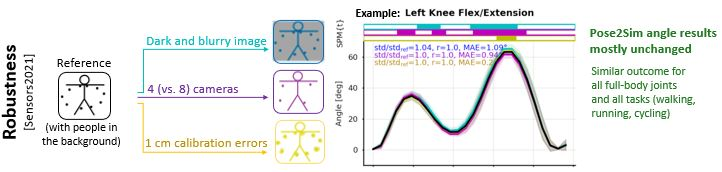
\includegraphics[width=\linewidth]{"../Intro/Figures/Fig_VisAbstract2.JPG"}
      \caption{Visual abstract for Pose2Sim robustness assessment \cite{Pagnon2021}.}
	\label{fig_visabstract2}
\end{figure}

\newpage


\section{Introduction}
\subsection{Robustness definition}

According to the review of \cite{Desmarais2021}, the performance of a method can be ranked regarding its accuracy, speed, or robustness. Accuracy is mostly assessed with MPJPE (Mean Per Joint Position Error); speed is evaluated either regarding computing complexity, or framerate when possible; and robustness is gauged through differences in the results while changing the system parameters only. \cite{Desmarais2021} points out that authors usually only consider accuracy, sometimes speed, but rarely robustness. However, robustness is of paramount importance in the context of sports, especially "in the wild". This chapter will focus on robustness, the next one on \nameref{ch:5}, and we will not focus on speed in this thesis (although chapter 3.4.5 broaches \hyperref[subsec:realtime]{Real time considerations}).

\cite{Moeslund2001} proposed to express robustness as the number of constraints on the subject or on the environment required for a motion capture system to be operational. Some of the assumptions they proposed have already been universally overcome by deep-learning-based methods. For example, no markers are involved anymore, the subject can wear their usual clothes (including loose pants or dresses \cite{Viswakumar2019}), and the background does not need to be static or uniform. Some other items remain an open problem.

For instance, most 3D methods assume that only one person lies in the camera field of view. This is a strong assumption, especially outdoors where people and athletes pass by and an operator is often present. Although it is starting to be addressed, standard solutions are yet to be determined \cite{Slembrouck2020,Bridgeman2019, Chu2021, Dong2019}. 

Other open questions lie in the environment, much less controlled in a sports context than in a lab, which can result in poor image qualities. \cite{Viswakumar2019} experienced that OpenPose is very robust to extreme lighting conditions. However, research has shown that pose estimations models are more robust to noise or brightness changes, while less robust to motion or to defocus blur \cite{Wang2021b}. And yet, in sports, the movement is not usually slow, continuous, nor limited to the sagittal plane.

Occlusions are, for the most part, solved by using a network of calibrated cameras. Since triangulation is computed using a least square method, a large amount of cameras will also blunt imprecision on the 2D joint estimations. \cite{Bala2020} showed that once correctly trained for 3D macaque pose estimation, eight cameras were enough to correctly infer 80\% of the 13 considered keypoints, while four cameras decreased the performance to about 50\%. However, a correct estimation of extremities such as feet and hands required more than eight cameras.

Camera calibration can be challenging outside, due to large volume spaces, bright light, and contrasting shades. As a consequence, it is close to impossible with the classic approach using a wand equipped with retro-reflective markers. Moreover, simple calibration with a checkerboard may cause errors on intrinsic and extrinsic camera parameters estimation \cite{Sun2005}. A calibration is generally considered acceptable if the average residuals of each camera (i.e., the root mean square error of the reprojection of the 3D reconstructed coordinates on the 2D image plane) is below 1 pixel. In metric terms, the markers-based Qualisys Track Manager software recommends redoing a calibration when the average residuals exceed 3 millimeters \cite{Qualisys2018}. The pinhole camera model gives an equivalence between pixel values on the image plane, and metric values on the object plane at the center of the scene, as demonstrated by Figure~\ref{fig_pixmeterscorrespondance} and Equation~\ref{eqn:errobjimg}. See Chapter 2.2.1 on \nameref{subsec:Pinhole model} or \cite{Dawson-Howe1994} for in-depth explanations.

\begin{figure}[!ht]
	\centering
	\def\svgwidth{1\columnwidth}
	\fontsize{10pt}{10pt}\selectfont
	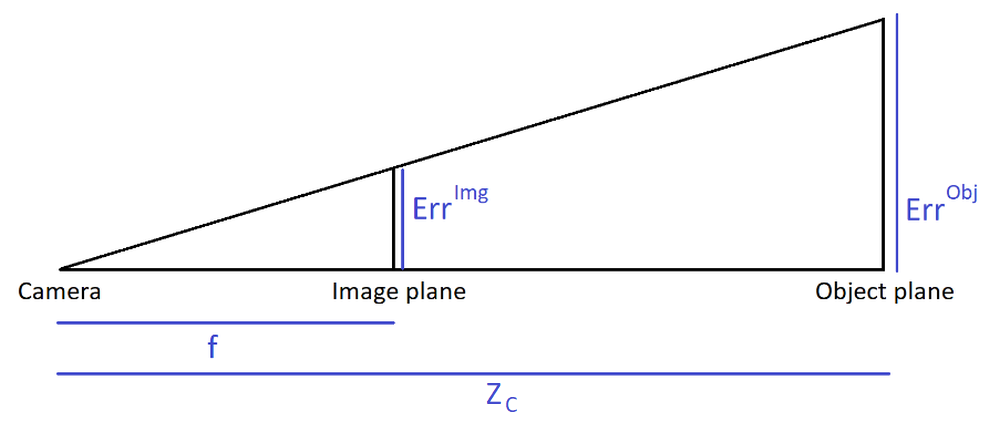
\includegraphics[width=0.6\linewidth]{"../Chap4/Figures/Fig_PixelMeterCorrespondance.png"}
	\caption{The pinhole camera model permits a correspondence between image coordinates and object coordinates. $f$: focal distance, $Z_C$: object to camera distance, $Err^{Img}$: error on image plane, $Err^{Obj}$: error on object plane. $f$ and $Err^{Img}$ are usually expressed in pixels, while $Z_C$ and $Err^{Obj}$ are expressed in meters.}
	\label{fig_pixmeterscorrespondance}
\end{figure}

\begin{equation}
      Err^{Img} = \frac{f \times Err^{Obj}}{Z_C} 
      \label{eqn:errobjimg}
\end{equation}


\subsection{Assessing robustness}

Because \cite{Needham2021a} showed that the quality of markerless results were task specific, we will examine walking, running, and cycling. Before assessing the robustness of the workflow, the relevance of the computed 3D full-body angles needs to be estimated. This will be done by comparing our angle results to those of a normative walking database. Further concurrent validation of the accuracy will be determined in the next chapter on \nameref{ch:5}. Assuming that the gait of a young and healthy person is repeatable, we assume that most of the variability between cycles should be caused by a lack of repeatability of the system. Thus, repeatability will be evaluated by comparing the kinematics of between cycles, within each task and each capture condition. 

Robustness itself will be assessed through all three types of movements, in accordance with the open problems previously described. In addition to the person of interest, some people will be present in the background in all examined conditions. We will compare results more in depth when:
\begin{enumerate}[itemsep=0em, topsep=0em]
      \item Image quality is altered, by simulating a dark scene captured with defocused cameras objectives.
      \item Self- and bike-occlusions are becoming more challenging, as we decrease the number of cameras.
      \item Calibration errors are introduced, by corrupting the calibration files.
\end{enumerate}

The underlying idea presented in this article is to verify whether modifying external environment parameters significantly impacts variability in joint angle estimation.

\section{Methods}

\href{https://github.com/davidpagnon/These_David_Pagnon/blob/main/Thesis/Chap4/Figures/Vid_Protocol.mp4?raw=true}{See video here} for a visual description of the protocol.

\subsection{Experimental setup}

To guarantee a tight control of the environment parameters, we captured our data in a dedicated studio platform called Kinovis \cite{Tsiminaki2014}, from which we were able to create realistic virtual views similar to outdoor video. This platform is a \(10 m \times 10 m \times 5.6 m\) green room equipped with 68 video cameras recording at 30 fps in 4 Mpixels resolution, for a practical acquisition space of about \(5 m  \times 5 m  \times 3 m\). The system computes 3D textured meshes by convex visual hull reconstruction \cite{Laurentini1994}. The meshes were inserted in a virtual environment composed of an environment texture map captured from a BMX racetrack, and a custom-made virtual floor. It should be noted that three people were present in the background, which introduced a realistic artifact of multiple subjects.

We developed a script for Autodesk Maya \cite{Maya1998} (see \nameref{subsec:viztools}) that allows us to render the textured mesh files, as well as to virtually set any cameras with specific properties (position, orientation, resolution, focal length, distortion, pixel size, binning factor). Views seen through virtual cameras can be saved as video files and visualized into a global 3D environment (Figure~\ref{fig_kinovis}). The generated video files were used as input to the 3D kinematics pipeline.

\begin{figure}[!ht]
	\centering
	\def\svgwidth{1\columnwidth}
	\fontsize{10pt}{10pt}\selectfont
	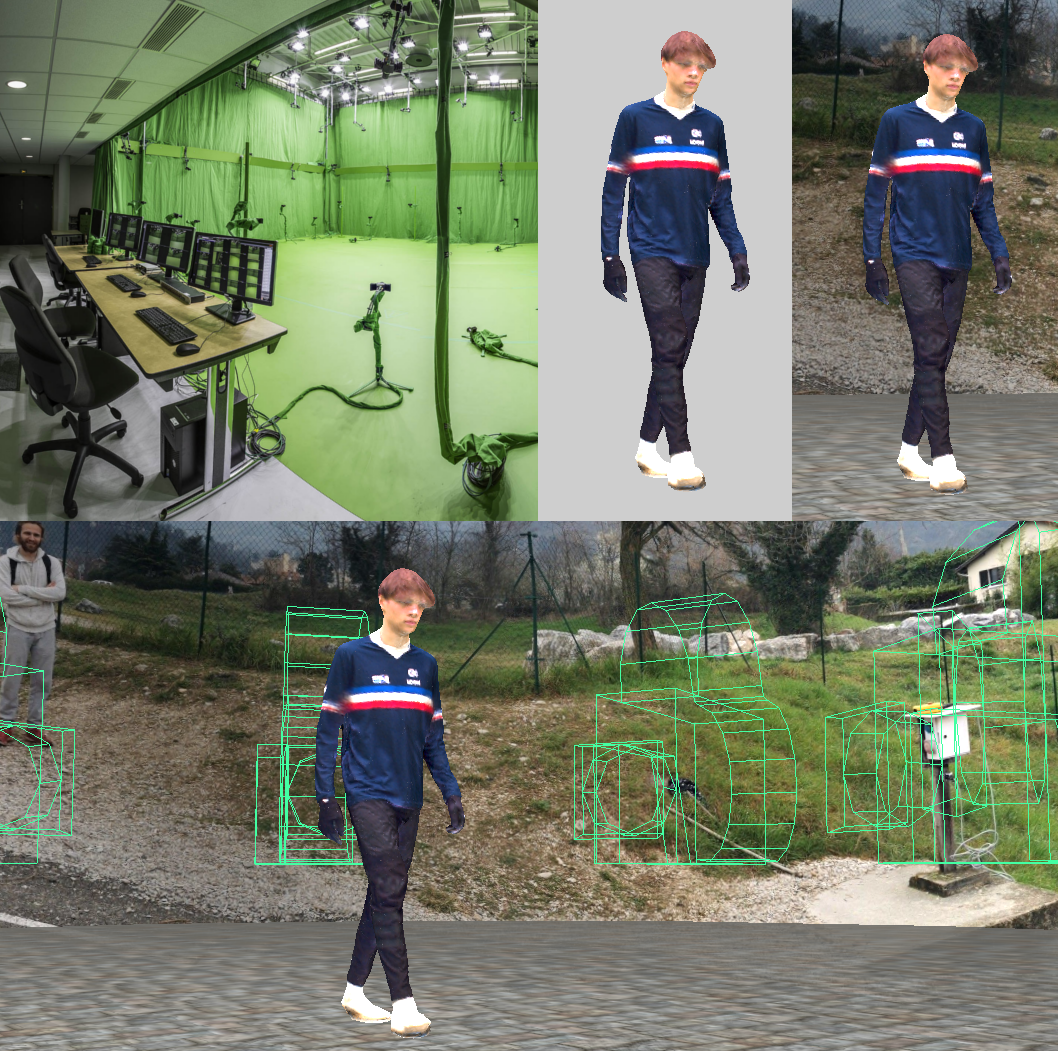
\includegraphics[width=\linewidth]{"../Chap4/Figures/Fig_Kinovis.png"}
	\caption{The Kinovis room allows for the capture of 3D textured meshes. These meshes are placed in a virtual environment, and then filmed from virtual cameras.}
	\label{fig_kinovis}
\end{figure}

For the purpose of this study, we created 8 virtual video cameras. Resolution was set to \(1280 \times 768\) pixels, focal length to 9 mm, pixel size to 5.54 µm, and no distortion nor binning was introduced. Binning refers to the process of grouping pixels in order to increase sensitivity to light, at the expense of decreasing resolution. Cameras were regularly distributed 8 m away from the center of the captured volume, at a height of 1 m, so that the whole body could be detected for a maximum of movement cycles. We then rendered the scene as video files from our virtual cameras and saved the exact calibration parameters. We applied a \(3 \times 3\) pixel Gaussian blur afterwards to reduce sharp edges of the virtual scene compositing (Figure~\ref{fig_smooth}). This resulting image quality was considered as “standard”.

\begin{figure}[!ht]
	\centering
	\def\svgwidth{1\columnwidth}
	\fontsize{10pt}{10pt}\selectfont
	\includegraphics[width=.95\linewidth]{"../Chap4/Figures/Fig_Smooth.png"}
	\caption{To smooth out sharp edges due to compositing, we applied a \(3 \times 3\) pixel Gaussian blur to the videos filmed from our virtual scene.}
	\label{fig_smooth}
\end{figure}


\subsection{Participant and protocol}

One healthy adult male subject (1.89 m, 69 kg) participated in the study. He provided his informed written consent prior to participating. The study was conducted in accordance with the Declaration of Helsinki \cite{Holm2013}. No requirement was given to him regarding his outfit. He was asked to perform three basic sports tasks: walking, running, and cycling. For all three tasks, the subject was given a moment beforehand to warm up and find a comfortable and regular pace, which he could then follow owing to the sound of a metronome:

\begin{itemize}[itemsep=0em, topsep=0em, leftmargin=*]
      \item \textit{Walking:} The subject walked in a straight line back and forth over the 10 m diagonal of the room. His body mesh could be fully reconstructed only in the central 5 m of the acquisition space, i.e., only roughly 2 gait cycles were acquired per walking line. His comfortable stride pace was 100 BPM (Beats per Minute). The stride length was not monitored. 
      \item \textit{Running:} The subject jogged in a straight line back and forth along the 10m diagonal of the room. His comfortable stride pace was 150 BPM (Beats per Minute). The stride length was not monitored.
      \item \textit{Cycling:} The subject cycled on a road bike placed on a home trainer. He himself adjusted the resistance and the height of the saddle prior to the capture. His comfortable cadence was 60 BPM.
\end{itemize}
As obtaining the textured meshes of the subject in the green Kinovis room involved filming simultaneously with 68 4 Mpixels cameras that generated a flow of over 8 gigabytes per second, the capture design limited the acquisition time to 45 s.


\subsection{Challenging robustness}

We challenged robustness with 3 challenging conditions, compared to a reference one.

\begin{itemize}[itemsep=0em, topsep=0em, leftmargin=*]
      \item \textit{Reference Condition (Ref):} The reference condition under which our 3D markerless kinematic system had to operate took advantage of the standard image quality, 8 available virtual cameras, and a perfect calibration. The standard quality corresponded to the unaltered images of the 3D scene filmed from our virtual cameras. The reference condition involved 8 virtual cameras, as a good compromise of what is feasible in real outdoor conditions. As a comparison, a study on macaques in a similar context showed that 8 cameras were enough to correctly infer 80\% of the 13 considered keypoints \cite{Bala2020}. Since the virtual cameras were explicitly specified in the virtual environment, calibration could be considered perfect.
      \item \textit{Poor Image Quality (Im):} Video quality was made blurrier and darker: a Gaussian blur (\(11 \times 11 px\)) was applied, as well as a 0.5 gamma compression (Figure~\ref{fig_imquality}). This simulated a dark scene captured with defocused camera objectives. These parameters were chosen empirically.
      \item \textit{Less Cameras (4c):} The 2D joint coordinates were triangulated with only 4 cameras, instead of 8 in the reference condition: one on each side, one in the front, and one in the back, set 90° apart from each other.
      \item \textit{Calibration Errors (Cal):} Calibration residuals are classically supposed to be under 1 px on the image plane or under 3 mm on the object plane. Using Equation~\ref{eqn:errobjimg} demonstrates that in our case 3 mm corresponds to 0.61 px. We chose to simulate a calibration error of 2 px, which corresponds to about 1 cm (Equation~\ref{eqn:errobjcal}).
      \begin{equation}
            Err^{Obj} = \frac{Err^{Img} \times D}{f} = \frac{2 \times 8}{\frac{9 \times 10^{-3}}{5.54 \times 10^{-6}}} = 9.8 \times 10^{-3} m
            \label{eqn:errobjcal}
      \end{equation} 
      The calibration error was simulated by translating the extrinsic parameters of each camera in a random direction. The norm was randomly picked in a normal distribution of mean 2 px and a standard deviation of 1 px. The mean of these 8 translations was ensured to be equal to \(2 ± 10^{-3}\) px.
\end{itemize}

\begin{figure}[!ht]
	\centering
	\def\svgwidth{1\columnwidth}
	\fontsize{10pt}{10pt}\selectfont
	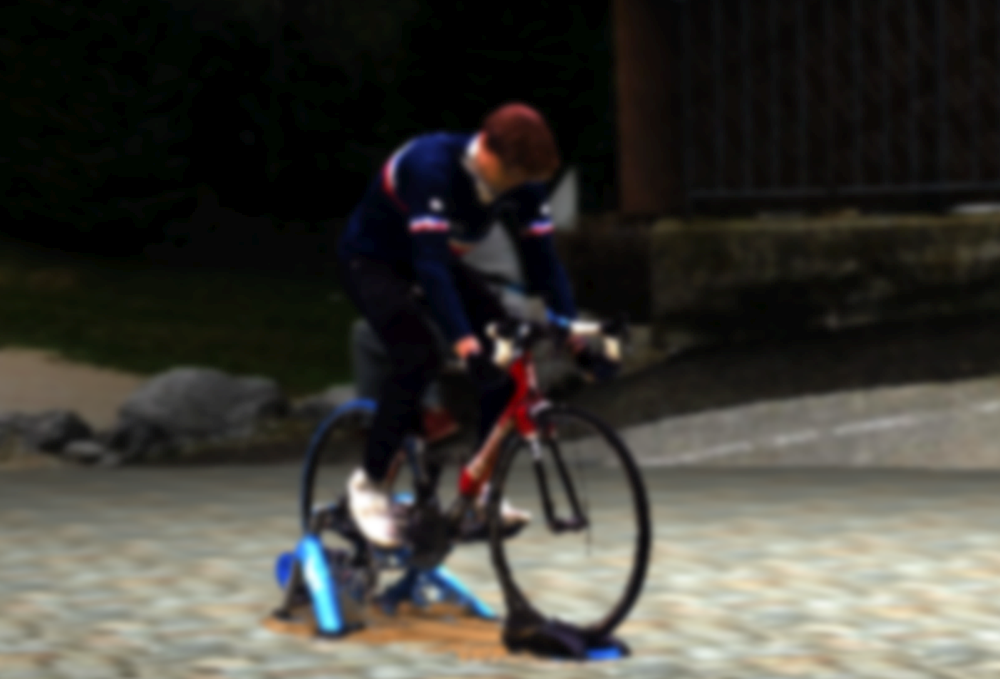
\includegraphics[width=\linewidth]{"../Chap4/Figures/Fig_ImQuality.png"}
	\caption{The image under poor image quality (Im) conditions. A Gaussian blur (\(11 \times 11 px\)) was applied, and a 0.5 gamma compression made the image darker.}
	\label{fig_imquality}
\end{figure}


\subsection{Markerless kinematics}

Then, we used Pose2Sim to robustly triangulate OpenPose outputs and feed the resulting 3D joint coordinates to OpenSim. The exact same parameters were used for all 4 conditions and all 3 movement tasks, in order to make sure the process did not induce any supplementary deviation to the compared results.

\subsubsection{2D pose estimation}

We applied OpenPose (version 1.6) on all the captured videos. We used the experimental body\_25B model (see~Figure\ref{fig_body25b}) with highest accuracy parameters, which is more accurate than the default body\_25 one and reduces the number of false positives \cite{Hidalgo2019}.

\subsubsection{Tracking, triangulation, and filtering}

We used the Tracking function of Pose2Sim to try out every possible triangulation of the neck keypoint of all detected persons. The person with the smallest reprojection error was deemed to be the one to be tracked. If the reprojection error was above 10 pixels, one camera was removed and the process was repeated. See \nameref{tracking} Chapter 3 for more details.

The weighted DLT provided by the Triangulation function of Pose2Sim was employed. Some keypoints were sometimes occluded to some cameras, either by the subject himself, by his cycling gear, or simply because the subject left the camera field of view. In such a case, OpenPose usually gave a low (or zero) confidence to the estimated point, which was dealt with by setting a confidence threshold above which the camera in question was not used for the triangulation. However, OpenPose occasionally wrongly detected the occluded keypoint with a relatively high confidence. Under such circumstances, the point was erroneously triangulated. This issue was spotted and solved by reprojecting the 3D point on the camera planes. If the reprojection error between the reprojected points and the OpenPose detection was higher than a predefined threshold, the process was repeated after removing one, or several, cameras. If less than 3 cameras remained, the frame was dropped for this point, and missing frames were later interpolated with a cubic spline. 3D joints positions were then exported as an OpenSim compatible .trc file.
We chose a confidence threshold of 0.3 and a reprojection error threshold of 10 px.

3D coordinates were finally filtered with a Butterworth filter \cite{Butterworth1930}. We chose a zero-lag fourth order low-pass Butterworth filter, with a 6 Hz cutoff frequency.

\subsubsection{Gait events determination}

Cycles were determined using one of the methods given by \cite{Zeni2008} for the determination of gait events using kinematic data. Zeni et al. suggested defining heel strike as the time of maximum distance between the heel and the sacrum. Here, the sacrum marker was assimilated to the ipsilateral hip joint coordinate. Although there is no heel strike in cycling, we used the same definition as a reference for the start of a cycle. An implementation of the algorithm is provided by Pose2Sim in \href{https://github.com/perfanalytics/pose2sim/blob/main/Pose2Sim/Utilities/trc_gaitevents.py}{Utilities/trc\_gaitevents.py}. A cycle was defined as starting from heel strike, with a duration \(t_{cycle}\):
\begin{equation}
      t_{cycle} = \frac{2}{cadence/60}seconds
\end{equation}

The duration of a cycle \(t_{cycle}\) was 1.2 s for walking, 0.8 s for running, and 1.0 s for cycling. The reduced area of acquisition and the limit of 45 s of capture restricted the analysis to 8, 9, and 15 cycles for walking, running, and cycling, respectively.


\subsubsection{Kinematic analysis}

The full-body musculo-skeletal model proposed by \cite{Rajagopal2016} was adjusted to our needs. OpenPose model markers were carefully placed on the body, as closely as possible to their average triangulated 3D coordinates. Muscles were removed since they were not considered at that stage. A ball joint was added between head and torso so that the rotation of the head could be roughly rendered. Pelvis translation and subtalar angle rotation were unlocked. Lumbar extension and lumbar bending were clamped between -15° and 15°, and constraints on hip flexion/extension ranges of motion were released since they were too strict for our cycling task. This model uses a coupling relationship between knee flexion and the other planes of movement, which allows for 3D knee kinematics with only one degree of freedom. \textit{Note that the model was later improved when assessing the accuracy of the workflow.}

See previous chapter on \nameref{ch:3} for more details on the scaling and inverse kinematics procedures. We visually verified at the end of the inverse kinematic step that model markers approximately overlaid experimental markers (Figure~\ref{fig_opensim}), and we batched inverse kinematics for all gait cycles with the command line utilities. We then concatenated all results in a .csv file analyzed them using python.

\begin{figure}[!ht]
	\centering
	\def\svgwidth{1\columnwidth}
	\fontsize{10pt}{10pt}\selectfont
	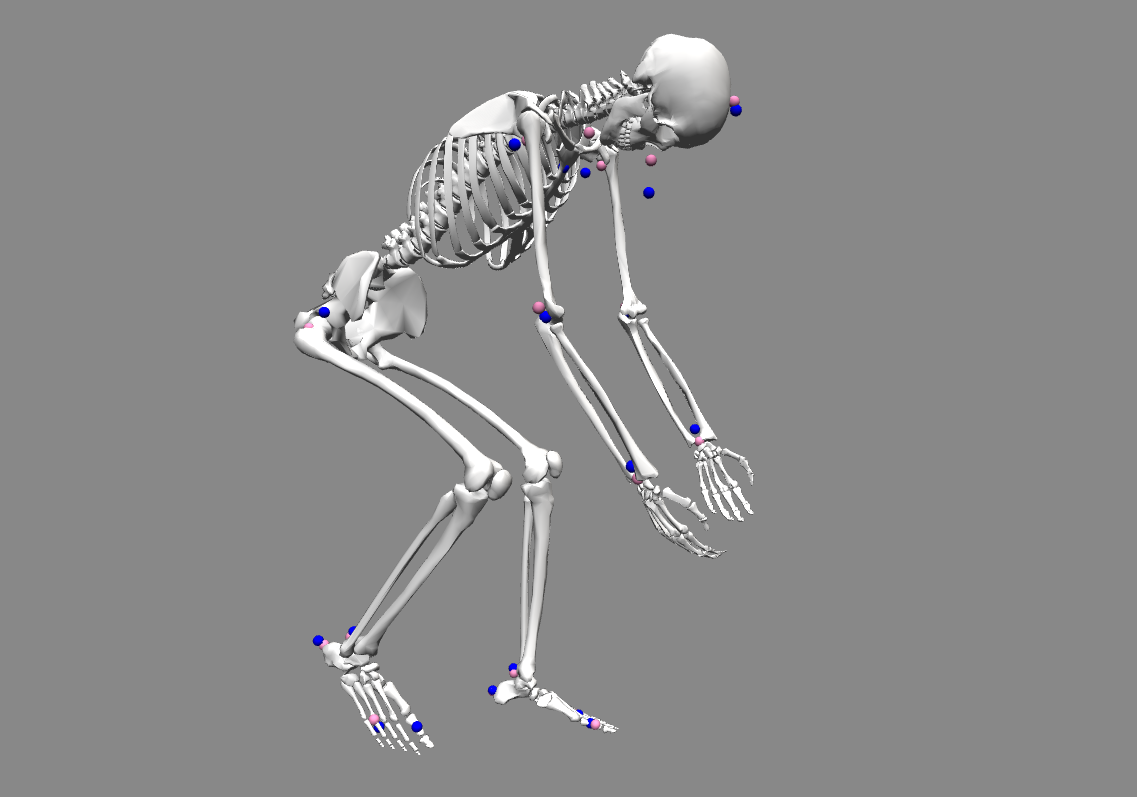
\includegraphics[width=\linewidth]{"../Chap4/Figures/Fig_OpenSim.png"}
	\caption{OpenSim inverse kinematics on cycling (C). Model markers are pink; experimental markers are blue.}
	\label{fig_opensim}
\end{figure}

\subsection{Statistical analysis}

As similar results were expected for both sides, as more strides were captured on the left one, and for the sake of clarity, the analysis was performed on the left side only. Descriptive statistics were calculated at the triangulation stage, for each (Ref), (Im), (4c), and (Cal) condition. We calculated mean, standard deviation (std), and maximum (max) number of cameras excluded for performing triangulation. Triangulation was deemed acceptable in Pose2Sim when OpenPose confidence was above 0.3, and when reprojection error was below 10 pixels. We also calculated mean, std, and max reprojection errors. Descriptive statistics of the OpenSim scaling and inverse kinematics steps were also rendered: we retrieved mean, std, and max root-mean-square error (RMSE) of the experimental and model markers.

Next, we investigated the relevance of our results. The angles of the Ref condition on the walking task were compared to those of a normative walking gait database \cite{Fukuchi2018}, from which we took a subset of 14 young and healthy males walking at a "comfortable" speed (Norm). Pearson’s correlations (r) and mean absolute error (MAE) were calculated. As the angle definition was different from that in the OpenSim model \cite{Trinler2019}, only the flexion/extension angles were compared.

Repeatability was estimated by computing stride-to-stride standard deviations within (Ref), (Im), (4c), and (Cal) conditions. These stride-to-stride variability results were then compared to \cite{Kang2008}, obtained with a marker-based approach and averaged over 18 young adults. The robustness of the workflow was assessed by calculating the standard deviation ratio between each degraded condition and the Ref one, as well as the r coefficient and the MAE. Statistical parametric analysis (SPM-1D) was lastly performed between Ref and degraded conditions to convey statistical differences along time (See \cite{Warmenhoven2018}).


\section{Results}
\subsection{Data collection and 2D pose estimation}
Each trial took several hours to process on a cluster of high-end computation units. Then, filming the resulting 3D meshes in a virtual scene with virtual cameras also took a few hours per sequence, as well as about 50 Go of storage space. Although all of this allowed us to perfectly control the parameters of the capture, this step would not be carried out in the wild, where capture would simply be carried out by filming with calibrated cameras.

Apart from the capture design, which is very particular to this study, the OpenPose 2D pose estimation was the most computationally costly step. On a standard computer with an Nvidia GeForce GTX 1080 graphic card (8 Go memory), the detection for each camera ran at a little over 0.5 fps (i.e., 0.07 fps for 8 cameras).


\subsection{Pose2Sim tracking, triangulation, and filtering}

On our standard computer, tracking was performed at an average of 5 fps depending on the number of undesired persons present in the background; triangulation was at about 10 fps; and filtering was almost instantaneous in comparison.

Depending on the considered frame, the reprojection error of a joint coordinate sometimes exceeded the prescribed threshold. In this case, the triangulation process was executed another time after excluding the 2D joint coordinates estimated from one, or several, cameras. Over all frames, an average of approximately 0.5 cameras were excluded in walking and in running and 1.6 in cycling (Table~\ref{table:tab_descstat}). The mean of the reprojection error was about 3.5 px ($\approx$1.6 cm) in walking and running and 6 px ($\approx$3 cm) in cycling. More cameras had to be excluded for the nose and for the extremities such as wrists and toes, and the reprojection error was mostly large on hips, head, and extremities.

\begin{table}[!ht]
      \resizebox{\textwidth}{!}{
      \centering
      \begin{tabular}{llllllll}
      \toprule
          \multirow{2}{*}{\textbf{Task}} & \multirow{2}{*}{\textbf{Conditions}} & \multicolumn{3}{c}{\shortstack{\textbf{Mean number of} \\\textbf{excluded cameras}}} & \multicolumn{3}{c}{\shortstack{\textbf{Mean absolute} \\\textbf{reprojection error}}} \\ 
          \cmidrule(l{2pt}r{2pt}){3-5}\cmidrule(l{2pt}r{2pt}){6-8}
          ~ & ~ & mean & std & max & mean & std & max \\ 
          \specialrule{0.14 em}{0pc}{0pc}
          \multirow{4}{*}{Walking} & Ref & 0.47 & 0.57 & 2.0 (Nose) & 3.3 px (1.6 cm) & 1.1 px (0.54 cm) & 5.3 px (2.6 cm, LHip) \\ 
          & Im & 0.91 & 0.8 & 2.4 (LWrist) & 3.7 px (1.8 cm) & 1.0 px (0.52 cm) & 5.2 px (2.6 cm, LSmallToe) \\
          & 4c & 0.27 & 0.34 & 1.0 (Nose) & 2.9 px (1.4 cm) & 0.93 px (0.47 cm) & 4.5 px (2.2 cm, LSmallToe) \\
          & Cal & 0.47 & 0.57 & 2.0 (Nose) & 5.1 px (2.5 cm) & 0.91 px (0.45 cm) & 6.9 px (3.4 cm, LHip) \\ 
          \midrule
          \multirow{4}{*}{Running} & Ref & 0.48 & 0.64 & 2.2 (LWrist) & 3.5 px (1.7 cm) & 1.2 px (0.57 cm) & 5.6 px (2.8 cm, LWrist) \\
          & Im & 0.94 & 1.2 & 4.5 (LWrist) & 4.0 px (2.0 cm) & 1.4 px (0.69 cm) & 7.2 px (3.6 cm, RWrist) \\ 
          & 4c & 0.22 & 0.31 & 1.0 (LWrist) & 3.3 px (1.6 cm) & 0.97 px (0.48 cm) & 4.7 px (2.3 cm, LWrist) \\
          & Cal & 0.47 & 0.65 & 2.2 (LWrist) & 5.4 px (2.7 cm) & 1.0 px (0.52 cm) & 7.2 px (3.6 cm, LWrist) \\
          \midrule
          \multirow{4}{*}{Cycling} & Ref & 1.62 & 1.4 & 4.2 (RBigToe) & 6.1 px (3.0 cm) & 1.2 px (0.58 cm) & 8.5 px (4.2 cm, Head) \\
          & Im & 2.41 & 1.9 & 5.7 (RBigToe) & 6.3 px (3.1 cm) & 1.3 px (0.60 cm) & 8.5 px (4.2 cm, Head) \\ 
          & 4c & 0.76 & 0.67 & 2.1 (RBigToe) & 5.3 px (2.6 cm) & 1.6 px (0.82 cm) & 8.4 px (4.2 cm, LElbow) \\
          & Cal & 1.68 & 1.4 & 4.24 (RBigToe) & 6.9 px (3.4 cm) & 1.0 px (0.51 cm) & 8.9 px (4.4 cm, Head) \\ 
      \bottomrule
      \end{tabular}}
      \caption{Descriptive statistics on the triangulation step performed by Pose2Sim from OpenPose body\_25B model. Mean absolute reprojection error and mean number of excluded cameras were calculated over time. Mean (mean), standard deviation (std), and maximum (max) in each of these variables are displayed. Walking, running, and cycling tasks were investigated in each four conditions: reference (Ref), poor image quality (Im), four cameras instead of eight (4c), and calibration errors (Cal).}
	\label{table:tab_descstat}
  \end{table}

Within each task, almost twice as many cameras had to be excluded in the (Im) condition as in the (Ref) condition, with nearly one camera excluded in walking and running, and nearly 2.5 in cycling. However, the reprojection error was increased by only about 10\%. About twice as few cameras had to be excluded in the (4c) condition as in (Ref) condition, and the reprojection error was decreased by about 10\%. The (Cal) condition did not involve more excluded cameras; indeed, calibration errors had no effect on the OpenPose confidence, and reprojection error stayed within the threshold of 10 px. However, a 2 px average error in calibration logically resulted in about a 2 px ($\approx$1 cm) larger reprojection error than in the Ref condition.


\subsection{OpenSim scaling and inverse kinematics}

Scaling took a few hours, which is in line with the usual expectations in marker-based methods. However, markers would be positioned in the same place by the pose estimation algorithm regardless of the subject and of the operator: as a consequence, in the future, only bones would have to be scaled, and markers will not have to be further adjusted. Due to the small number of markers whose positions had to be optimized, Opensim’s inverse kinematics ran at more than 0.5 fps.

OpenSim recommends the RMS of experimental vs. model marker errors to be below 1 cm for scaling. Our best average RMS error was 1.9 cm. During inverse kinematics, it is recommended for it to stay below 2–4 cm. The average RMS error was typically below 4 cm, but it could reach much more for some markers at certain phases of the cycle, especially in the cycling task. Within each task, changing conditions made very little difference in RMS marker errors, including in mean, standard deviation (std), or maximum error (Table~\ref{table:tab_opensim}).

\begin{table}[!ht]
      \centering
      \begin{tabular}{lllll}
      \toprule
          \multirow{2}{*}{\textbf{Task}} & \multirow{2}{*}{\textbf{Condition}} & \multicolumn{3}{c}{\textbf{RMS marker error}} \\ 
          \cmidrule{3-5}
          ~ & ~ & mean & std & max \\ 
          \specialrule{0.14 em}{0pc}{0pc}
          \multirow{4}{*}{Walking} & Ref & 2.8 cm & 0.13 cm & 3.2 cm (Mid stance) \\ 
          ~ & Im & 2.8 cm & 0.11 cm & 3.1 cm (Mid stance) \\ 
          ~ & 4c & 2.8 cm & 0.12 cm & 3.2 cm (Mid stance) \\ 
          ~ & Cal & 2.9 cm & 0.13 cm & 3.2 cm (Mid stance) \\ 
          \midrule
          \multirow{4}{*}{Running} & Ref & 2.2 cm & 0.22 cm & 2.6 cm (Mid stance) \\ 
          ~ & Im & 2.4 cm & 0.21 cm & 2.8 cm (Mid stance) \\ 
          ~ & 4c & 2.5 cm & 0.30 cm & 2.4 cm (Mid stance) \\ 
          ~ & Cal & 2.2 cm & 0.21 cm & 2.6 cm (Mid stance) \\ 
          \midrule
          \multirow{4}{*}{Cycling} & Ref & 3.4 cm & 0.11 cm & 3.6 cm (Dead center) \\ 
          ~ & Im & 3.8 cm & 0.18 cm & 4.2 cm (Dead center) \\ 
          ~ & 4c & 3.9 cm & 0.60 cm & 5.9 cm (Dead center) \\ 
          ~ & Cal & 3.4 cm & 0.11 cm & 3.6 cm (Dead center) \\ 
      \bottomrule
      \end{tabular}
      \caption{Descriptive statistics on the inverse kinematics step performed by OpenSim with a full body model adapted from Rajagopal’s. Root mean square (RMS) errors between experimental and model markers were calculated over all markers. Mean, standard deviation (std), and maximum (max) are displayed. Dead center refers to the phase where the crank is near the vertical position.}
      \label{table:tab_opensim}
  \end{table}

Note that one should not compare the values of the reprojection errors in the triangulation step, and of the marker errors in the inverse kinematics one. Primarily, the first one is calculated over time, while the second one is calculated over markers. Additionally, the first one is a mean absolute error (MAE), while the second one is a root mean square error (RMSE). RMSE squares the errors, which always makes it larger than the MAE. It penalizes large errors more, which has some implications that are not addressed here but are documented in \cite{Chai2014}. These errors should only be used to compare conditions within each step.


\subsection{Relevance, repeatability and robustness of angles Results}

Flexion/extension lower-limb angles were compared to a normative walking gait database \cite{Trinler2019} (Figure~\ref{fig_compnorm}). Ankle movement differed noticeably (r = 0.35, MAE = 5.4°), especially between 40\% and 70\% of the gait cycle. There was a good agreement for the knee (r = 0.93, MAE = 5.7°) and hip angles (r = 0.97, MAE = 9.0°) despite some notable offset in hip angle. A similar shift occurred in the pelvis ante/retroversion angle (not further analyzed).

\begin{figure}[!ht]
	\centering
	\def\svgwidth{1\columnwidth}
	\fontsize{10pt}{10pt}\selectfont
	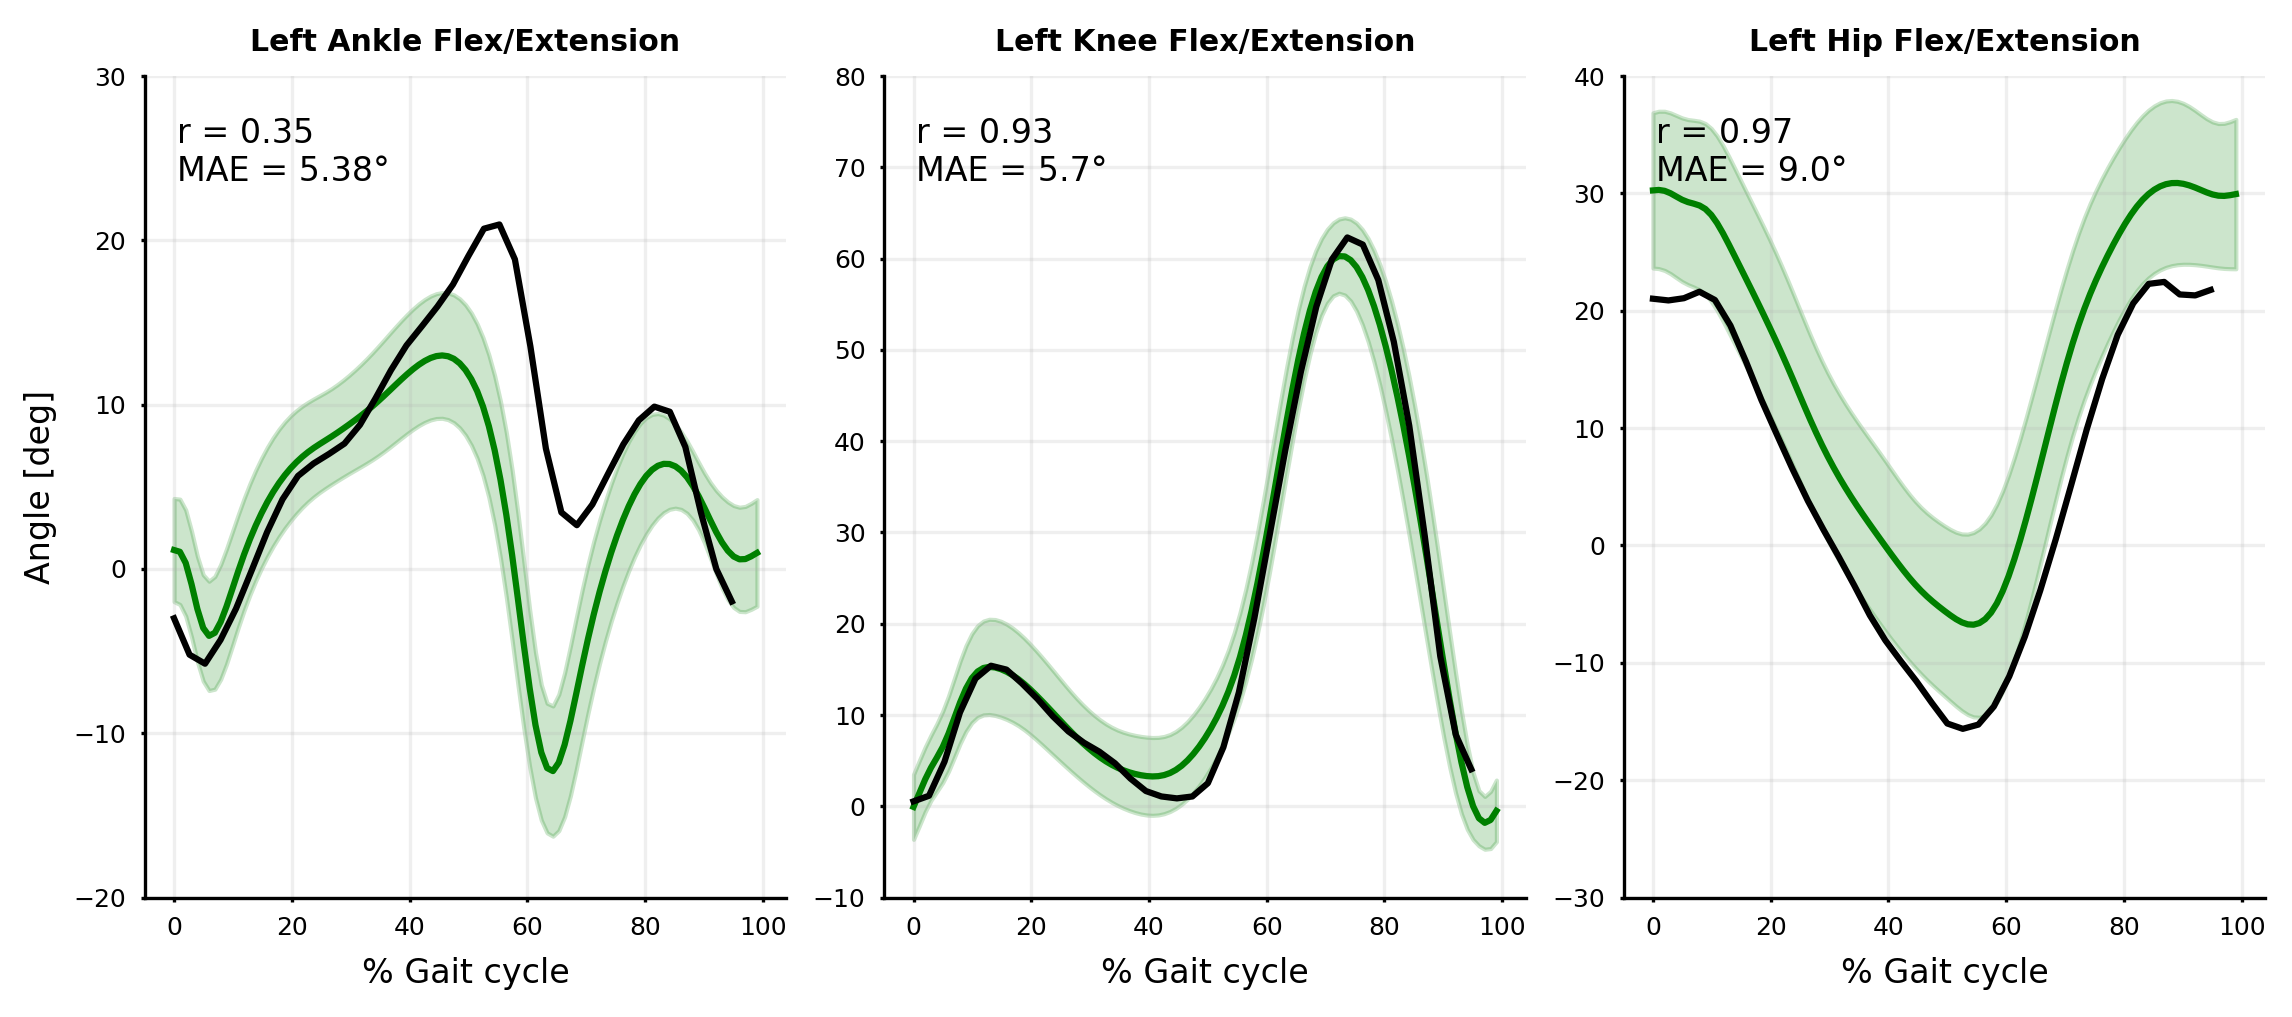
\includegraphics[width=\linewidth]{"../Chap4/Figures/Fig_CompNorm.png"}
	\caption{Comparison between our markerless results (black line: mean stride-to-stride results for our subject) and the normative marker-based database (green line and area: mean and standard deviation across 14 young, healthy, male subjects). Mean absolute error (MAE) and Pearson correlation coefficient (r) are represented.}
	\label{fig_compnorm}
\end{figure}

\newpage
When averaged over all joint angles, the stride-to-stride standard deviations lay between 1.7° and 3.2° for all conditions and tasks (Table~\ref{table:tab_sumstats}). The walking task was the most variable, while the cycling one was the least variable; however, in the latter the upper body was static and artificially drew the mean down, which was revealed after removing it from the statistics (Table~\ref{table:tab_sumstats}). In the walking task, the stride-to-stride standard deviation of our individual lower body angles was higher than \cite{Kang2008}, who used a marker-based approach (Table~\ref{table:tab_comp_mk}).

\begin{table}[!ht]
      \centering
      \begin{tabular}{llllll}
          \toprule
          \textbf{Task} & \textbf{Condition} & \textbf{std (°)} & \textbf{std/stdref} & \textbf{r} & \textbf{MAE (°)} \\ 
          \specialrule{0.14 em}{0pc}{0pc}
          \multirow{4}{*}{Walking} & Ref & 2.56 & - & - & - \\ 
          ~ & Im & 3.03 & 1.19 & 0.97 & 1.55 \\ 
          ~ & 4c & 3.24 & 1.27 & 0.97 & 1.50 \\ 
          ~ & Cal & 2.60 & 1.02 & 1.00 & 0.35 \\ 
          \midrule
          \multirow{4}{*}{Running} & Ref & 2.59 & - & - & - \\ 
          ~ & Im & 2.76 & 1.07 & 0.99 & 0.92 \\ 
          ~ & 4c & 2.79 & 1.10 & 0.97 & 1.60 \\ 
          ~ & Cal & 2.54 & 0.98 & 1.00 & 0.47 \\ 
          \midrule
          \multirow{4}{*}{Cycling} & Ref & 1.78 & - & - & - \\ 
          ~ & Im & 1.89 & 1.08 & 0.88 & 1.72 \\ 
          ~ & 4c & 3.04 & 1.93 & 0.81 & 1.54 \\ 
          ~ & Cal & 1.80 & 1.02 & 0.99 & 0.50 \\ 
          \midrule
          \multirow{4}{*}{\shortstack{Cycling \\(lower-body only)}} & Ref & 2.09 & - & - & - \\ 
          ~ & Im & 2.41 & 1.22 & 0.94 & 1.69 \\ 
          ~ & 4c & 3.82 & 2.31 & 0.90 & 1.84 \\ 
          ~ & Cal & 2.13 & 1.03 & 0.99 & 0.51 \\ 
          \bottomrule
      \end{tabular}
      \caption{Summary of angles statistics, averaged for all joints. Each condition is represented: reference condition (Ref), degraded image quality (Im), four cameras instead of eight (4c), degraded calibration (Cal). Comparisons between each Im, 4c, Cal conditions, and Ref are accounted for with standard deviation (std), the standard deviation ratio (std/stdref), the Pearson’s correlation coefficient (r), and the mean absolute error (MAE).}
      \label{table:tab_sumstats}
\end{table}

\begin{table}[!ht]
      \centering
      \begin{tabular}{lllll}
          \toprule
          \textbf{Joint} & \textbf{Method} & \textbf{Flexion/Extension} & \textbf{Abduction/Adduction*} & \textbf{Internal/External rotation} \\ 
          \specialrule{0.14 em}{0pc}{0pc}
          \multirow{2}{*}{Ankle} & \cite{Kang2008}   & 2 & 2.5 & - \\ 
          ~ & \textbf{Ours} & \textbf{2.07} & \textbf{4.84} & \textbf{-} \\ 
          \midrule
          \multirow{2}{*}{Knee} & \cite{Kang2008}    & 0.7 & - & - \\ 
          ~ & \textbf{Ours} & \textbf{4.85} & \textbf{-} & \textbf{-} \\ 
          \midrule
          \multirow{2}{*}{Hip} & \cite{Kang2008}  & 1.2 & 1.8 & 1.1 \\ 
          ~ & \textbf{Ours} & \textbf{2.61} & \textbf{1.5} & \textbf{3.72} \\ 
          \bottomrule
      \end{tabular}
      \caption{Stride-to-stride standard deviations of lower-body angles. Comparison between our markerless approach, and a marker-based one (averaged over 18 young subjects). * Ankle subtalar angle is assimilated to an abduction/adduction angle.}
      \label{table:tab_comp_mk}
\end{table}

There was a good agreement between the Ref condition and the degraded ones, at the same time across all tasks, movement planes, and joints. Mean absolute errors (MAE) averaged over all joint angles (compared to the reference condition—Ref) ranged between 0.35° and 1.7° for all conditions and tasks (Table~\ref{table:tab_sumstats}). Individual angle MAE lay between 0.07° and 5.2° (Figure~\ref{fig_walkrobust} for the walking task, and Figure~\ref{fig_runrobust} and Figure~\ref{fig_bikerobust} in the Appendix for the running and cycling tasks). However, the cycling task was more challenging: ankle joint angles were especially less robust regarding all considered dependent variables.

\begin{figure}[!ht]
	\centering
	\def\svgwidth{1\columnwidth}
	\fontsize{10pt}{10pt}\selectfont
	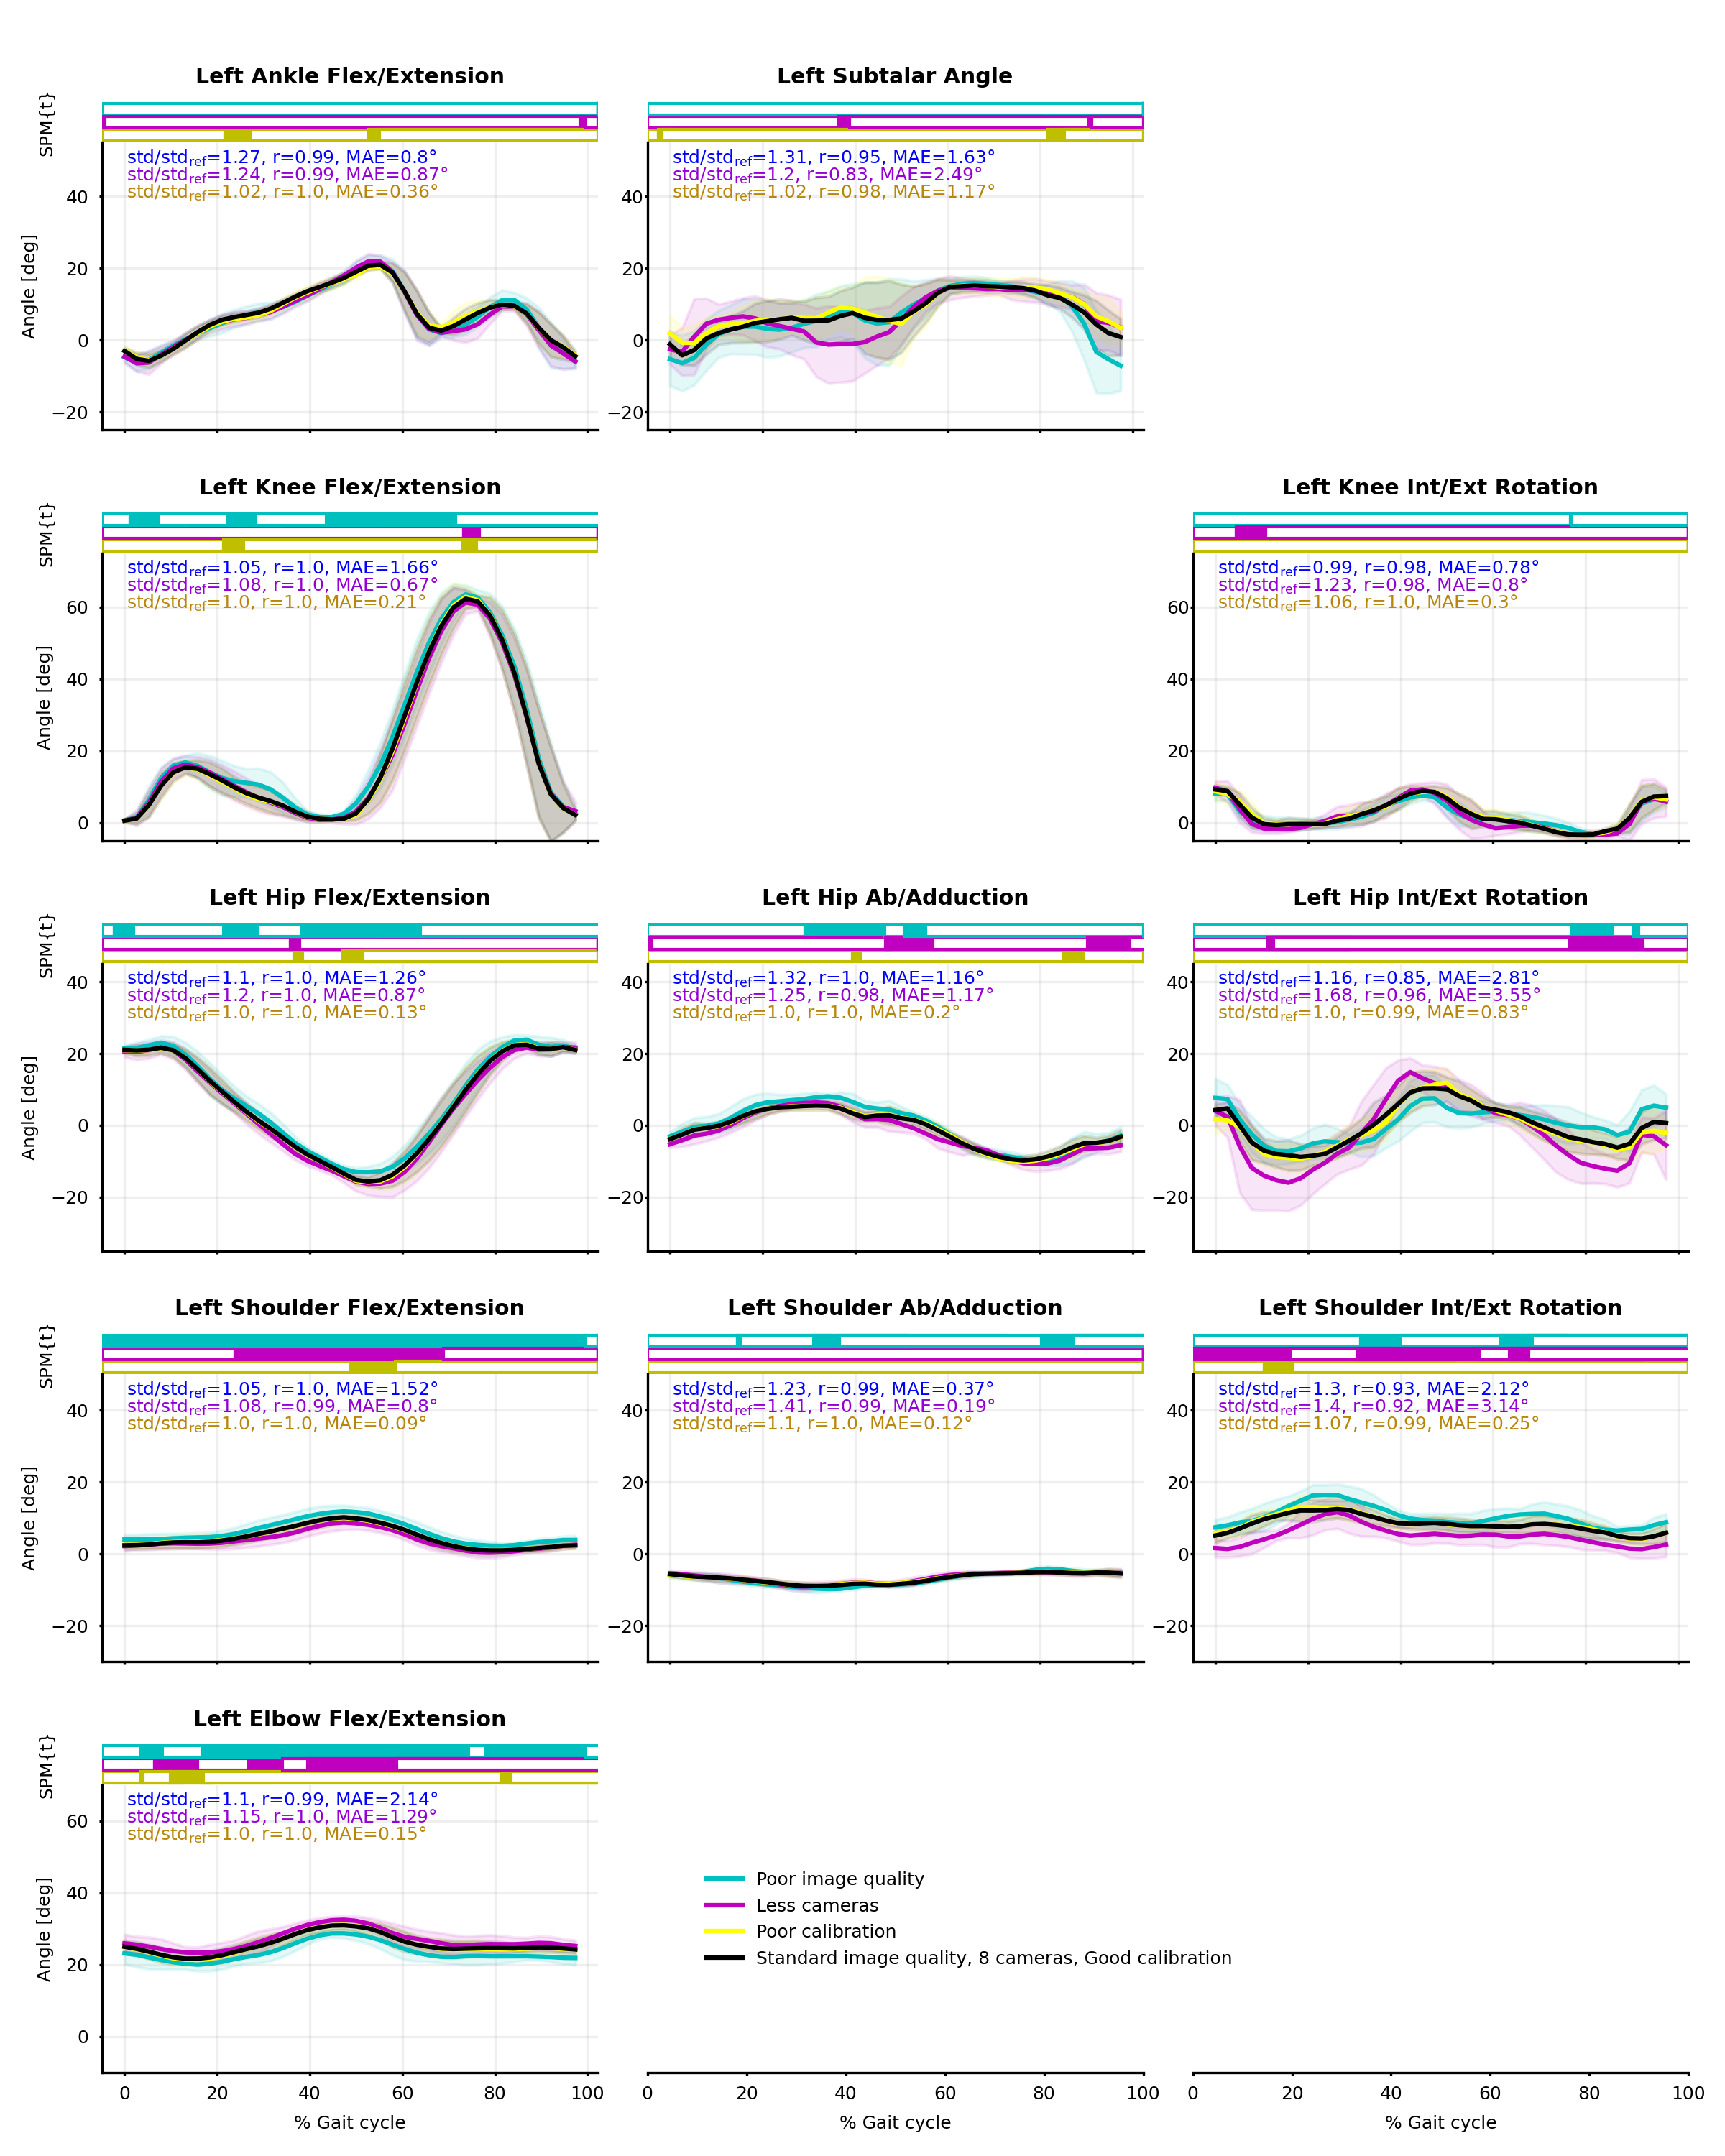
\includegraphics[height=\dimexpr\textheight-119pt]{"../Chap4/Figures/Fig_WalkRobust.png"}
	\caption{Joint angle means (solid line) and standard deviations (shaded area) from the eight captured cycles of walking. Reference condition (Ref) is black; degraded image quality (Im) is blue; four cameras instead of eight (4c) is purple; degraded calibration (Cal) is yellow. Pearson’s correlation coefficient (r) and mean absolute error (MAE) between Ref and Im, 4c, Cal are reported. Paired t-tests along time were computed by SPM-1D and are represented as bar plots above the curves: a color rectangle means that there was a cluster of statistically significant differences (\(\alpha\) = 0.05) at that moment. Running and cycling figures can be found in the Supplementary Material.}
	\label{fig_walkrobust}
\end{figure}

Angle results were particularly little affected by the 1 cm calibration error (Cal condition). The standard deviation between cycles (std) virtually did not increase, the average Pearson’s r correlation coefficient was 1.00 in all tasks but the cycling one (r = 0.98), and the mean absolute angle error stayed below 0.5° (Table~\ref{table:tab_sumstats}).

The standard deviation in Im and 4c conditions increased by about 10 to 30\% as compared to Ref condition, apart from the cycling 4c condition where it increased by 100\%. The Pearson’s r correlation coefficient was about 0.98 in all tasks but the cycling one. Mean absolute angle errors across all joints lay between 0.9 and 1.8° (Table~\ref{table:tab_sumstats}).

\clearpage
Kinematics were more robust in the flexion/extension plane (Table~\ref{table:tab_statsperplane}), where std generally did not increase by more than 10\% as compared to the Ref condition, and r was mostly equal to 1.00. The difference in robustness was not as obvious in the MAE variable since the range of motion was much smaller in other planes.

\begin{table}[!ht]
      \resizebox{\textwidth}{!}{
      \centering
      \begin{tabular}{lllllllllll}
          \toprule
              \multirow{2}{*}{\textbf{Task}} & \multirow{2}{*}{\textbf{Cond.}} & \multicolumn{3}{c}{\textbf{ Flex./Ext.}} & \multicolumn{3}{c}{\textbf{Abd./Add.*}} & \multicolumn{3}{c}{\textbf{Int./Ext. rot.}}\\ 
                  \cmidrule(l{2pt}r{2pt}){3-5}\cmidrule(l{2pt}r{2pt}){6-8}\cmidrule(l{2pt}r{2pt}){9-11}
                  ~ & ~ &  \(\mathrm{std/std_{ref}}\) & r & MAE (°) &  \(\mathrm{std/std_{ref}}\) & r & MAE (°)&  \(\mathrm{std/std_{ref}}\) & r & MAE (°) \\ 
                  \specialrule{0.14 em}{0pc}{0pc}
                  \multirow{3}{*}{Walking} & Im	& 1.11&	1.00&	1.48&	1.28&	0.98&	1.05&	1.23&	0.89&	2.47 \\
                  &	4c&	1.15&	1.00&	0.90&	1.29&	0.93&	1.28&	1.54&	0.94&	3.35\\
                  &	Cal&	1.01&	1.00&	0.19&	1.04&	0.99&	0.50&	1.04&	0.99&	0.54\\
                  \midrule
                  \multirow{3}{*}{Running} & Im	& 1.03&   1.00&	0.98&	1.08&	0.98&	0.48&	1.13&	0.98&	1.41\\
                    &4c	&1.03&	1.00&	0.98&	1.18&	0.93&	1.00&	1.14&	0.97&	4.06\\
                    &Cal&	1.00&	1.00&	0.30&	0.99&	0.99&	0.53&	0.92&	1.00&	0.80\\
                  \midrule
                  \multirow{3}{*}{Cycling} & Im	& 0.99	&0.97&	1.89&	1.27&	0.66&	1.45&	0.99&	0.97&	1.71\\
                    &4c&	1.31&	0.96&	1.43&	3.10&	0.46&	1.76&	1.71&	0.97&	1.47\\
                    &Cal&	1.00&	1.00&	0.39&	1.06&	0.96&	0.36&	1.02&	1.00&	1.00\\
          \bottomrule
      \end{tabular}}
      \caption{Summary of angles statistics in the three rotation planes, averaged over all joints (n = 5, 3, 2 for Flexion/Extension, Abduction/Adduction, and Internal/External Rotation, respectively.). All conditions are represented: degraded image quality (Im), four cameras instead of eight (4c), and degraded calibration (Cal). These conditions were compared to the reference one (Ref) by calculating the ratio of standard deviation (std/stdref), the Pearson’s correlation coefficient (r), and the mean absolute error (MAE). *Ankle subtalar angle is assimilated to an abduction/adduction angle.}
      \label{table:tab_statsperplane}
\end{table}

The SPM showed some statistical differences along time between the reference condition and the degraded ones; however, they did not happen at any particular moment during the gait or pedaling cycle (Figure~\ref{fig_walkrobust} for the walking task, and Figure~\ref{fig_runrobust} and Figure~\ref{fig_bikerobust} in the Appendix for the running and cycling tasks).\newline

% \FloatBarrier
\section{Discussion}

% \subsection{Pose2Sim}

% Pose2Sim allows for seamless markerless kinematics from a network of calibrated and synchronized cameras by connecting two widespread, renowned, and open-source tools: the OpenPose 2D pose estimator and the OpenSim movement analysis software. Overall, human intervention is scarce, which makes it more robust to human error. Pose2Sim automatically tracks the person of interest when people are in the background, considers the confidence given by the OpenPose estimation, and is robust to missing frames and to the person exiting the field of view of one or several cameras. To the best of our knowledge, it is also the first one taking advantage of a solid anatomical 3D model in order to solve some rotations around the limb and to account for physical consistency. It is very customizable, in the sense that the user can adjust most parameters and even use a different 2D pose estimator if needed, including for non-human subjects (such as DeepLabCut \cite{Mathis2018} for example.)


\subsection{Relevance, repeatability and robustness}

Results of joint angles in the walking condition seemed to be realistic when compared to the normative database. The noticeable discrepancies may be due to a difference between the angle definition of both models, especially in the ankle: the normative database calculated 6 degrees-of-freedom free-body angles between limb segments, while our OpenSim model took bone geometries into consideration. The shift in the hip angle was related to an excessive pelvis anteversion, which may have been induced by the model being underconstrained due to OpenPose dearth of keypoints. This lack of marker constraints could be partly compensated by adding joint constraints, especially around the spine (See next chapter on \nameref{ch:5}, combining the \cite{Rajagopal2016} and the \cite{Beaucage-Gauvreau2019} models). In any case, the angle results seem to be relevant, but accuracy needs to be further investigated by comparing Pose2Sim markerless method to a reference marker-based one exploiting a similar model definition.

\newpage
Repeatability was simply assessed by the standard deviation of angle time series across gait cycles, although it also includes the participant’s intrinsic variability. However, the subject being young and healthy, his gait and cycling patterns were thought to be consistent. Hence, the results were repeatable as the standard deviation of angles across all strides within all tasks and conditions mostly stayed below 3°. Nevertheless, this standard deviation was still higher than the one previously reported by \cite{Kang2008} for a young and healthy participant using a marker-based approach. It may be partly caused by our lack of a force plate and our low sampling rate, which did not let us measure a very accurate heel strike event, and thus could have induced some additional variability. In addition, our videos were sampled at 30 Hz instead of hundreds of Hertz as is usual in motion analysis. It is to be noted that high-speed video cameras can sample at a such speed and solve at least a part of this issue. Depending on the sports task investigated, a 3° standard deviation can be more or less of an issue.

Robustness was investigated based on the criteria exposed by \cite{Moeslund2001}. First, people could be in the background. Then, several movement tasks have been investigated. Last, the workflow was confronted to three degraded conditions regarding image quality, camera number, and calibration. The results were also robust, since degraded conditions still gave consistent joint angles. A further SPM study showed occasional statistical differences along time, but did not reveal any part of the movement cycle to be more problematic than another. There was no apparent outlier in the 3D angle results, even in the degraded conditions. This was in spite of the presence of other people in the field of view and in spite of the subject walking out of it.

All stages of the workflow contributed to its robustness. First, we never had to deal with limb swapping, unlike other studies \cite{Nakano2019,Slembrouck2020}. This may be due to our use of the experimental Body\_25B OpenPose model, which is claimed to decrease the number of false positives \cite{Hidalgo2019}. Then, we used Pose2Sim to robustly sort the detected people and to triangulate 2D coordinates. These coordinates were the least precise in the Im condition where the image was strongly blurred and darkened, but Pose2Sim partly solved it by taking the OpenPose likelihood into account and by excluding the most inaccurate cameras: twice as many cameras were excluded as compared to the reference condition, which resulted in a reprojection error only 10\% higher.

Finally, we used OpenSim to take advantage of a physically consistent full-body model and of an inverse kinematics optimization algorithm, which allowed us to refine our 3D data coordinates and to obtain 3D joint angles. The Cal condition simulated calibration errors, which bypassed the Pose2Sim safeguards since the OpenPose likelihood was unaffected, and the reprojection error stayed below the threshold. Despite it producing the largest reprojection error, virtually no difference with the reference condition was observed after the OpenSim pass. A 2 px calibration error ($\approx$1 cm) is much worse than the maximum 1 px, or 3 mm usually recommended, but the mean absolute error it induced for us stayed below 0.5°.

Using four cameras rather than eight still gave relevant angle results, but the individual errors of each camera cannot be blunted by the multiplicity of views, especially when faced with occlusion issues such as in the cycling task. The ankle joint angles were especially less robust regarding all considered dependent variables because the feet were more easily occluded by the cycling gear.

Ultimately, all conditions challenged the workflow at different stages, but the results remained stable and very close to those of the reference condition, with an average mean absolute error mostly lower than 1.5°, a correlation coefficient largely above 0.95, and a standard deviation usually increased by less than 20\%. This demonstrates the robustness of the presented method in conditions that would have probably caused marker-based approaches to fail. Moreover, our reported angle deviations seem quite reasonable compared to errors in marker-based approaches, which can propagate up to 10° because of inter-operator differences \cite{Croce1999,Gorton2009}, to 3° because of tissue artifacts \cite{Benoit2015,Cappozzo1995}, or to 3° depending on the joint center calculation method \cite{Leboeuf2019}. Essentially, the findings presented here seem to indicate that the slight decline in repeatability is an acceptable compromise when put into perspective with the increase in robustness, in ease of use, and in new opportunities for analysis of sports performed "in-the-wild".

Nonetheless, it would be interesting to check for even more challenging conditions. We have investigated global Gaussian blur, but not movement blur, such as when the camera shutter speed is not high enough. It would also be interesting to investigate the effect of even larger calibration errors, even less cameras used, different camera placements, different camera types (such as GoPros with strong fisheye distortions), or different framerates or image definitions.


\subsection{Limits and perspectives}

Our use of a virtual scene helped us perfectly control all parameters of the capture. Although this scene is synthetically crafted, it looks similar to a real one. This is not thought to hinder the performance of 2D pose detection since deep-learning models are occasionally trained on synthetic datasets that look empirically less real and still successfully transfer to real-world data (see \cite{Nikolenko2021,Patel2021,Wood2021,Bolanos2021,Varol2017}). However, an image with a better definition and with a framerate over 30 fps may improve results. Furthermore, the 68 video camera capture design uses up very large storage space, and the restricted space offered by the Kinovis room constrained us to capture only a few cycles per capture. This limited us to a low amount of data, with only one subject and about 10 cycles analyzed per task.

We noticed that the cycling task was particularly challenging, probably because of self-occlusions and gear occlusions. Setting some cameras closer to the ankles and in a lower position would have slightly improved this issue. Unlike \cite{D'Antonio2021}, we did not find running to be more challenging for our system than walking. In the context of sports sciences, it would be useful to test other tasks, such as boxing (a typical 3D movement, explored in chapter 6 on \nameref{ch:6} \cite{Pagnon2022c}), flipping (the 2D pose estimator may have trouble with upside-down people), swimming (in an environment with a different refractive index, with splashes around limb extremities), or a sport discipline with unusual outfits and large occlusions (such as motorbiking or fencing.)

Moreover, the \cite{Rajagopal2016} model used as a basis does not appear to be well suited for road cycling since the spine is designed as a single rigid bone that cannot bend. This results in sharp shifts in hip abduction/adduction and internal/external rotation angles, which are not biomechanically coherent (see Figure~\ref{fig_bikerobust}). However, the same issue would prevail even with marker-based methods and would only be solved by changing the spine definition in the OpenSim model. The full-body model with a fully articulated spine and ribcage developed by \cite{Bruno2015} has far too many degrees of freedom for our small amount of detected keypoints; however, the lifting full-body (LFB) model validated by \cite{Beaucage-Gauvreau2019} solved the spine challenge by constraining vertebra movements to each other, without adding any degrees of freedom. Pose2Sim now provides a combination of these two models (see \hyperref[ch:3]{Pose2Sim package}) in order to benefit from the most realistic options (assuming a healthy subject), both in the knee and in the spine. This is the one used in the next section on \nameref{ch:5}.

For further use in a sports context, it would also be useful to support multi-person analysis, to have a more accurate and extensive 2D pose estimator, to work in real time, and to provide a GUI. All these considerations are discussed in the \nameref{ch3_lim} section of the previous chapter on the \hyperref[ch:3]{Pose2Sim package}.

\cite{Desmarais2021} proposed a taxonomy of 3D pose estimation algorithms based on accuracy, speed, and robustness. Although more modalities could be tested, our workflow was robust in the range of our tested conditions. Speed was unaddressed, but although real-time analysis seems out of reach, a timely analysis of athletes' movements directly on the sports field appears to be achievable. Yet, ultimately, the accuracy of the workflow must be concurrently validated with a reference marker-based method. This is the topic of the next chapter.